% -*- coding: utf-8 -*-
%-------------------------designed by zcf--------------
\documentclass[UTF8,a4paper,10pt]{ctexart}
\usepackage[left=3.17cm, right=3.17cm, top=2.74cm, bottom=2.74cm]{geometry}
\usepackage{amsmath}
\usepackage{graphicx,subfig}
\usepackage{float}
\usepackage{cite}
\usepackage{caption}
\usepackage{enumerate}
\usepackage{booktabs} %表格
\usepackage{multirow}
\usepackage{minted}
\usemintedstyle{xcode}
\usepackage{svg}
\newcommand{\tabincell}[2]{\begin{tabular}{@{}#1@{}}#2\end{tabular}}  %表格强制换行
%-------------------------字体设置--------------
% \usepackage{times} 
\usepackage{ctex}
\setCJKmainfont[ItalicFont=Noto Sans CJK SC Bold, BoldFont=Noto Serif CJK SC Black]{Noto Serif CJK SC}
\newcommand{\yihao}{\fontsize{26pt}{36pt}\selectfont}           % 一号, 1.4 倍行距
\newcommand{\erhao}{\fontsize{22pt}{28pt}\selectfont}          % 二号, 1.25倍行距
\newcommand{\xiaoer}{\fontsize{18pt}{18pt}\selectfont}          % 小二, 单倍行距
\newcommand{\sanhao}{\fontsize{16pt}{24pt}\selectfont}  %三号字
\newcommand{\xiaosan}{\fontsize{15pt}{22pt}\selectfont}        % 小三, 1.5倍行距
\newcommand{\sihao}{\fontsize{14pt}{21pt}\selectfont}            % 四号, 1.5 倍行距
\newcommand{\banxiaosi}{\fontsize{13pt}{19.5pt}\selectfont}    % 半小四, 1.5倍行距
\newcommand{\xiaosi}{\fontsize{12pt}{18pt}\selectfont}            % 小四, 1.5倍行距
\newcommand{\dawuhao}{\fontsize{11pt}{11pt}\selectfont}       % 大五号, 单倍行距
\newcommand{\wuhao}{\fontsize{10.5pt}{15.75pt}\selectfont}    % 五号, 单倍行距
%-------------------------章节名----------------
\usepackage{ctexcap} 
\CTEXsetup[name={,、},number={ \chinese{section}}]{section}
\CTEXsetup[name={(,)},number={\chinese{subsection}}]{subsection}
\CTEXsetup[name={,.},number={\arabic{subsubsection}}]{subsubsection}
%-------------------------页眉页脚--------------
\usepackage{fancyhdr}
\pagestyle{fancy}
\lhead{\kaishu \leftmark}
% \chead{}
\rhead{\kaishu 预备工作1}%加粗\bfseries 
\lfoot{}
\cfoot{\thepage}
\rfoot{}
\renewcommand{\headrulewidth}{0.1pt}  
\renewcommand{\footrulewidth}{0pt}%去掉横线
\newcommand{\HRule}{\rule{\linewidth}{0.5mm}}%标题横线
\newcommand{\HRulegrossa}{\rule{\linewidth}{1.2mm}}
%-----------------------伪代码------------------
\usepackage{algorithm}  
\usepackage{algorithmicx}  
\usepackage{algpseudocode}  
\floatname{algorithm}{Algorithm}  
\renewcommand{\algorithmicrequire}{\textbf{Input:}}  
\renewcommand{\algorithmicensure}{\textbf{Output:}} 
\usepackage{lipsum}  
\makeatletter
\newenvironment{breakablealgorithm}
  {% \begin{breakablealgorithm}
  \begin{center}
     \refstepcounter{algorithm}% New algorithm
     \hrule height.8pt depth0pt \kern2pt% \@fs@pre for \@fs@ruled
     \renewcommand{\caption}[2][\relax]{% Make a new \caption
      {\raggedright\textbf{\ALG@name~\thealgorithm} ##2\par}%
      \ifx\relax##1\relax % #1 is \relax
         \addcontentsline{loa}{algorithm}{\protect\numberline{\thealgorithm}##2}%
      \else % #1 is not \relax
         \addcontentsline{loa}{algorithm}{\protect\numberline{\thealgorithm}##1}%
      \fi
      \kern2pt\hrule\kern2pt
     }
  }{% \end{breakablealgorithm}
     \kern2pt\hrule\relax% \@fs@post for \@fs@ruled
  \end{center}
  }
\makeatother
%------------------------代码-------------------
\usepackage{xcolor} 
\usepackage{listings} 
\lstset{ 
breaklines,%自动换行
basicstyle=\small,
escapeinside=``,
keywordstyle=\color{ blue!70} \bfseries,
commentstyle=\color{red!50!green!50!blue!50},% 
stringstyle=\ttfamily,% 
extendedchars=false,% 
linewidth=\textwidth,% 
numbers=left,% 
numberstyle=\tiny \color{blue!50},% 
frame=trbl% 
rulesepcolor= \color{ red!20!green!20!blue!20} 
}
%------------超链接----------
\usepackage[colorlinks,linkcolor=black,anchorcolor=blue]{hyperref}
%------------------------TODO-------------------
\usepackage{enumitem,amssymb}
\newlist{todolist}{itemize}{2}
\setlist[todolist]{label=$\square$}
% for check symbol 
\usepackage{pifont}
\newcommand{\cmark}{\ding{51}}%
\newcommand{\xmark}{\ding{55}}%
\newcommand{\done}{\rlap{$\square$}{\raisebox{2pt}{\large\hspace{1pt}\cmark}}\hspace{-2.5pt}}
\newcommand{\wontfix}{\rlap{$\square$}{\large\hspace{1pt}\xmark}}
%------------------------水印-------------------
\usepackage{tikz}
\usepackage{xcolor}
\usepackage{eso-pic}

\newcommand{\watermark}[3]{\AddToShipoutPictureBG{
\parbox[b][\paperheight]{\paperwidth}{
\vfill%
\centering%
\tikz[remember picture, overlay]%
  \node [rotate = #1, scale = #2] at (current page.center)%
    {\textcolor{gray!80!cyan!30!magenta!30}{#3}};
\vfill}}}

%———————————————————————————————————————————正文———————————————————————————————————————————————
%----------------------------------------------
\begin{document}
\begin{titlepage}
  \begin{center}
    
\includegraphics[width=0.8\textwidth]{figure/NKU.png}\\[1cm]
    \textsc{\Huge \kaishu{\textbf{南\ \ \ \ \ \ 开\ \ \ \ \ \ 大\ \ \ \ \ \ 学}} }\\[0.9cm]
    \textsc{\huge \kaishu{\textbf{计\ \ 算\ \ 机\ \ 学\ \ 院}}}\\[0.5cm]
    % \textsc{\Large \textbf{预习报告}}\\[0.8cm]
    \HRule \\[0.9cm]
    { \LARGE \bfseries 预备工作1}\\[0.4cm]
    \HRule \\[2.0cm]
    \centering
    \textsc{\LARGE 丁屹\kaishu{\ \ \ \ }}\\[0.5cm]
    \textsc{\LARGE \kaishu{年级\ :\ 2020级}}\\[0.5cm]
    \textsc{\LARGE \kaishu{专业\ :\ 计算机科学与技术}}\\[0.5cm]
    % \textsc{\LARGE \kaishu{指导教师\ :\ XX}}\\[0.5cm]
    \vfill
    {\Large \today}
  \end{center}
\end{titlepage}
%-------------摘------要--------------
\newpage
\thispagestyle{empty}
\renewcommand{\abstractname}{\kaishu \sihao \textbf{摘要}}
\begin{abstract}

  \noindent  %顶格
  \textbf{\\\ 关键字:预处理器、编译器、汇编器、链接器、LLVM IR}\textbf{} \\\ \\\
\end{abstract}
%----------------------------------------------------------------
\tableofcontents
%----------------------------------------------------------------
\newpage
\watermark{60}{10}{NKU}
\setcounter{page}{1}

\section{概述}
本次实验将以编译器 clang 为研究对象,深入地探究语言处理系统的完整工作过程:
\begin{enumerate}
  \item 预处理器做了什么?
  \item 编译器做了什么?
  \item 汇编器做了什么?
  \item 链接器做了什么?
  \item 通过编写 LLVM IR 程序,熟悉 LLVM IR 中间语言。
\end{enumerate}

以一个简单的计算斐波拉契数列的 C 源程序为例,调整编译器的程序选项获得各阶段的输出,研究它们与源程序的关系。

\begin{minted}[linenos,frame=lines]{c}
#include<stdio.h>
signed main() {
  int a, b, i, t, n;
  a = 0;
  b = 1;
  i = 1;
  scanf("%d%d%d", &n, &a, &b);
  while(i < n) {
    t = b;
    b = a + b;
    printf("%d\n", &b);
    a = t;
    i = i + 1;
  }
}
\end{minted}

\section{预处理器做了什么}
预处理过程扫描源代码,对其进行初步的转换,产生新的源代码提供给编译器。可见预处理过程先于编译器对源代码进行处理。在C语言中,并没有任何内在的机制来完成如下一些功能:在编译时包含其他源文件、定义宏、根据条件决定编译时是否包含某些代码。预处理过程读入源代码,检查包含预处理指令的语句和宏定义,并对源代码进行响应的转换。预处理过程还会删除程序中的注释和多余的空白字符。预处理指令是以\#号开头的代码行。\#号必须是该行除了任何空白字符外的第一个字符。\#后是指令关键字,在关键字和\#号之间允许存在任意个数的空白字符。整行语句构成了一条预处理指令,该指令将在编译器进行编译之前对源代码做某些转换。

对于 clang 编译器,使用命令 \verb|clang fib.c -E -o fib.i|,即可得到预处理后文件。

观察预处理文件,发现文件长度远大于源文件,再对比\verb|<stdio.h>|头文件定义内容,发现多出的部分即为头文件定义的具体内容。没有用到的头或注释则会被删去。 如对比图\ref{pic:1}所示。

\begin{figure}[H]
  \centering
  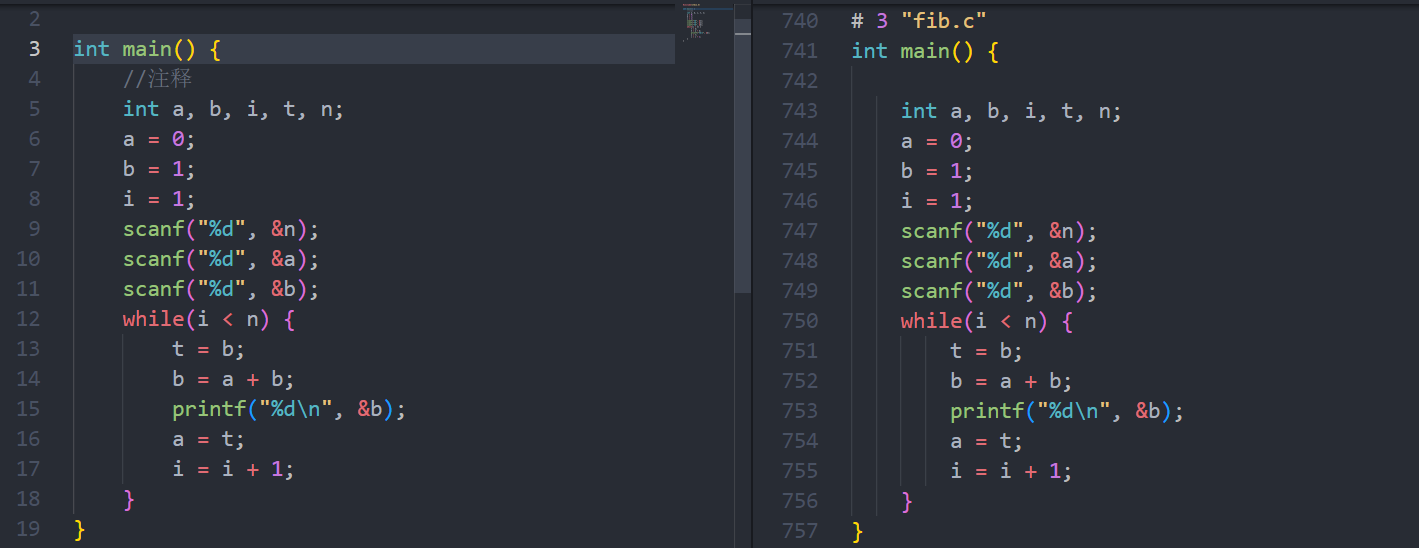
\includegraphics[width=\textwidth]{figure/diff1.png}
  \caption{左为源代码,右为经预处理器处理后的代码,可见行数增加且注释被删去。}
  \label{pic:1}
\end{figure}

\section{编译器做了什么}
\subsection{词法分析}
将源程序转换为单词序列,把代码切成一个个 token,比如大小括号、等于号、还有字符串等。对于 LLVM 编译器,通过以下命令获得 token 序列:\verb|clang -E -Xclang -dump-tokens fib.c|,部分输出如图\ref{pic:2}所示。

\begin{figure}[H]
  \centering
  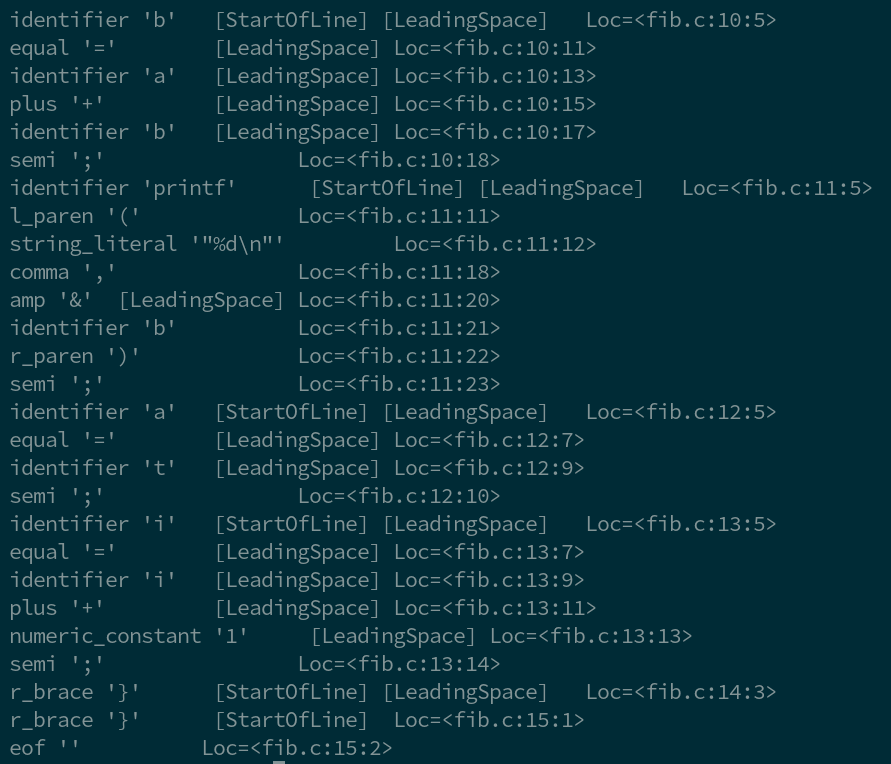
\includegraphics[width=\textwidth]{figure/token.png}
  \caption{token序列}
  \label{pic:2}
\end{figure}

\subsection{语法分析}
语法分析,它的任务是验证语法是否正确,在词法分析的基础上将单词序列组合成各类此法短语,如程序、语句、表达式 等等,然后将所有节点组成抽象语法树(Abstract Syntax Tree AST),语法分析程序判断程序在结构上是否正确。

对于 gcc,可以通过\verb|-fdump-tree-original-raw| flag 获得文本格式的 AST 输出。对于 LLVM 可以通过\verb|clang -E -Xclang -ast-dump fib.c|获得相应的 AST。此处我使用后者。部分输出如图\ref{pic:3}所示,可见明确树形结构。

\begin{figure}[H]
  \centering
  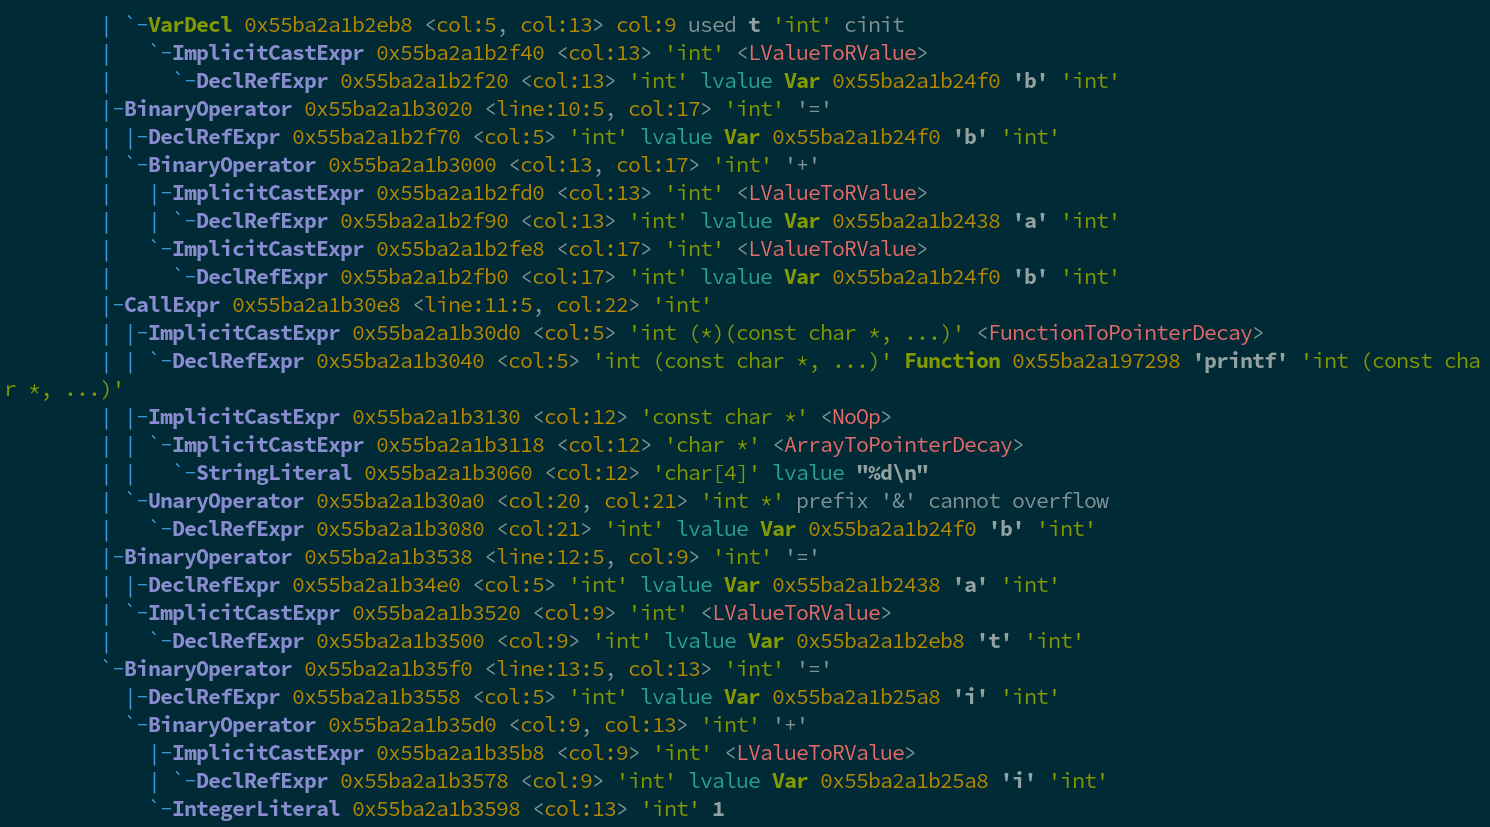
\includegraphics[width=\textwidth]{figure/AST.png}
  \caption{生成抽象语法树}
  \label{pic:3}
\end{figure}

\subsection{语义分析}
使用语法树和符号表中信息来检查源程序是否与语言定义语义一致,进行类型检查等。

\subsection{中间代码生成}
完成以上步骤后,就开始生成中间代码 IR 了,代码生成器会将语法树自顶向下遍历逐步翻译成 LLVM IR,可以通过下面命令可以生成 .ll 的文本文件,查看 IR 代码。

对于 GCC ,可以通过\verb|-fdump-tree-all-graph|和\verb|-fdump-rtl-all-graph|两个 gcc flag 获得中间代码生成的多阶段的输出。生成的 .dot 文件可以被 graphviz 可视化。如图\ref{pic:4}可以看到控制流图,以及各阶段处理中(比如优化、向 IR 转换)CFG 的变化。

LLVM 的优化级别分别是 -O0、-O1、-O2、-O3、-Os,下面是带优化的生成中间代码 IR 的命令:\verb|clang -Os -S -fobjc-arc -emit-llvm 源文件路径 -o 输出文件路径|

\begin{figure}[H]
  \centering
  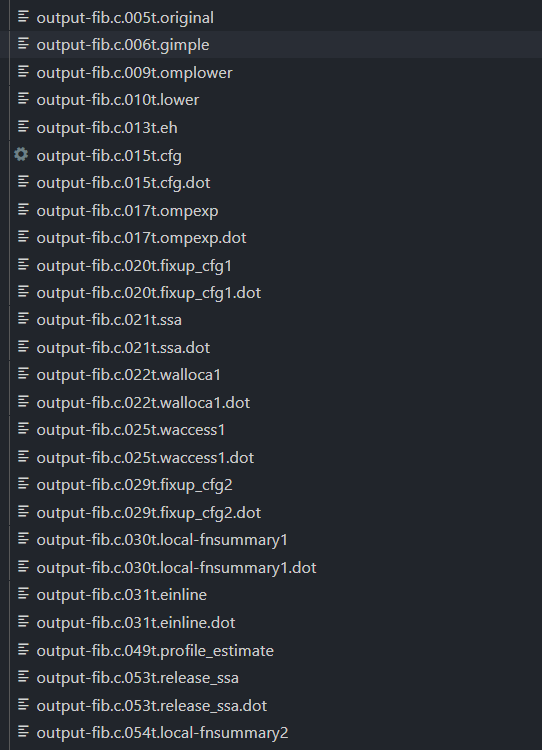
\includegraphics[width=\textwidth]{figure/gcc.png}
  \caption{控制流图}
  \label{pic:4}
\end{figure}

LLVM 可以通过下面的命令生成 LLVM IR:\verb|clang -S -emit-llvm fib.c|
\begin{minted}[linenos,frame=lines]{NASM}
; ModuleID = 'fib.c'
source_filename = "fib.c"
target datalayout = "e-m:e-p270:32:32-p271:32:32-p272:64:64-i64:64-f80:128-n8:16:32:64-S128"
target triple = "x86_64-pc-linux-gnu"

@.str = private unnamed_addr constant [3 x i8] c"%d\00", align 1
@.str.1 = private unnamed_addr constant [4 x i8] c"%d\0A\00", align 1

; Function Attrs: noinline nounwind optnone uwtable
define dso_local i32 @main() #0 {
  %1 = alloca i32, align 4
  %2 = alloca i32, align 4
  %3 = alloca i32, align 4
  %4 = alloca i32, align 4
  %5 = alloca i32, align 4
  %6 = alloca i32, align 4
  store i32 0, i32* %1, align 4
  store i32 0, i32* %2, align 4
  store i32 1, i32* %3, align 4
  store i32 1, i32* %4, align 4
  %7 = call i32 (i8*, ...) @__isoc99_scanf(i8* noundef getelementptr inbounds ([3 x i8], [3 x i8]* @.str, i64 0, i64 0), i32* noundef %6)
  %8 = call i32 (i8*, ...) @__isoc99_scanf(i8* noundef getelementptr inbounds ([3 x i8], [3 x i8]* @.str, i64 0, i64 0), i32* noundef %2)
  %9 = call i32 (i8*, ...) @__isoc99_scanf(i8* noundef getelementptr inbounds ([3 x i8], [3 x i8]* @.str, i64 0, i64 0), i32* noundef %3)
  br label %10

  10:                                               ; preds = %14, %0
  %11 = load i32, i32* %4, align 4
  %12 = load i32, i32* %6, align 4
  %13 = icmp slt i32 %11, %12
  br i1 %13, label %14, label %23

  14:                                               ; preds = %10
  %15 = load i32, i32* %3, align 4
  store i32 %15, i32* %5, align 4
  %16 = load i32, i32* %2, align 4
  %17 = load i32, i32* %3, align 4
  %18 = add nsw i32 %16, %17
  store i32 %18, i32* %3, align 4
  %19 = call i32 (i8*, ...) @printf(i8* noundef getelementptr inbounds ([4 x i8], [4 x i8]* @.str.1, i64 0, i64 0), i32* noundef %3)
  %20 = load i32, i32* %5, align 4
  store i32 %20, i32* %2, align 4
  %21 = load i32, i32* %4, align 4
  %22 = add nsw i32 %21, 1
  store i32 %22, i32* %4, align 4
  br label %10, !llvm.loop !6

  23:                                               ; preds = %10
  %24 = load i32, i32* %1, align 4
  ret i32 %24
}

declare i32 @__isoc99_scanf(i8* noundef, ...) #1

declare i32 @printf(i8* noundef, ...) #1

attributes #0 = { noinline nounwind optnone uwtable "frame-pointer"="all" "min-legal-vector-width"="0" "no-trapping-math"="true" "stack-protector-buffer-size"="8" "target-cpu"="x86-64" "target-features"="+cx8,+fxsr,+mmx,+sse,+sse2,+x87" "tune-cpu"="generic" }
attributes #1 = { "frame-pointer"="all" "no-trapping-math"="true" "stack-protector-buffer-size"="8" "target-cpu"="x86-64" "target-features"="+cx8,+fxsr,+mmx,+sse,+sse2,+x87" "tune-cpu"="generic" }

!llvm.module.flags = !{!0, !1, !2, !3, !4}
!llvm.ident = !{!5}

!0 = !{i32 1, !"wchar_size", i32 4}
!1 = !{i32 7, !"PIC Level", i32 2}
!2 = !{i32 7, !"PIE Level", i32 2}
!3 = !{i32 7, !"uwtable", i32 1}
!4 = !{i32 7, !"frame-pointer", i32 2}
!5 = !{!"Debian clang version 14.0.6-2"}
!6 = distinct !{!6, !7}
!7 = !{!"llvm.loop.mustprogress"}

\end{minted}

\subsection{代码优化}
进行与机器无关的代码优化步骤,此处通过 LLVM 现有的优化 pass 优化步骤改进中间代码,生成更好的目标代码。

pass 的分类共分为三种:Analysis Passes、Transform Passes 和 Utility Passes。Analysis Passes 用于分析或计算某些信息,以便给其他 pass 使用,如计算支配边界、控制流图的数据流分析等;Transform Passes 都会通过某种方式对中间代码形式的程序做某种变化,如死代码删除,常量传播等。

通过下面的命令生成每个 pass 后生成的 LLVM IR,以观察区别:

\verb|llc -print-before-all -print-after-all fib.ll > fib.log 2>&1|

对输出重定向到 fib.log 中,部分生成代码对比如图\ref{pic:5}所示:
\begin{figure}[H]
  \centering
  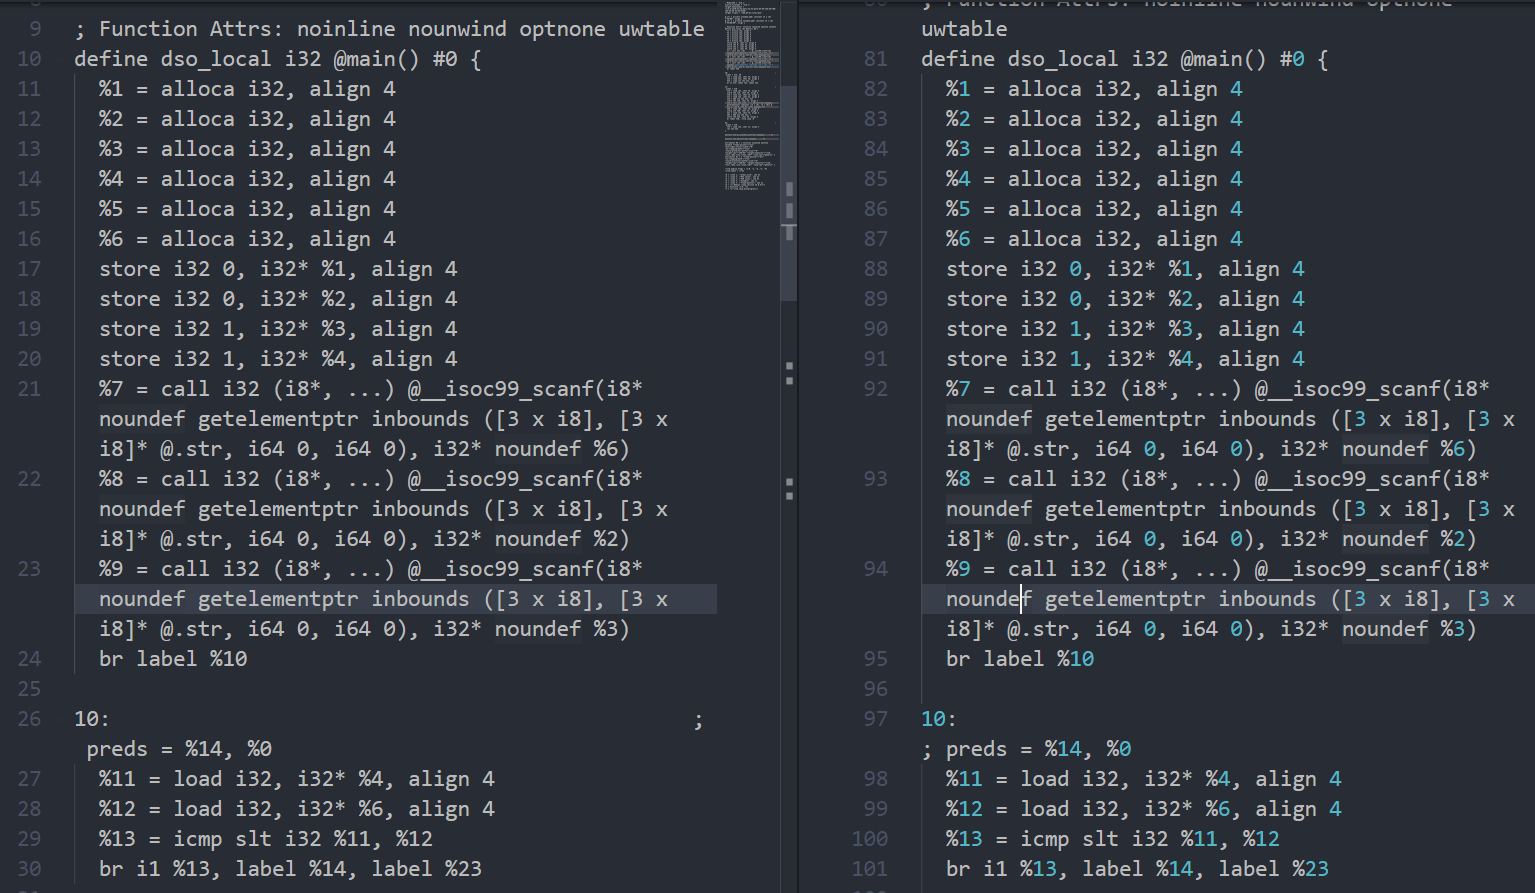
\includegraphics[width=\textwidth]{figure/diff2.png}
  \caption{左为fib.ll,右为fib.log}
  \label{pic:5}
\end{figure}

\subsection{代码生成}
以中间表示形式作为输入,将其映射到目标语言。
此处我使用 LLVM 生成。

\begin{minted}[linenos,frame=lines]{shell}
    gcc fib.i -S -o fib.S # 生成 x86 格式目标代码
    arm-linux-gnueabihf-gcc fib.i -S -o fib.S # 生成 arm 格式目标代码
    llc fib.ll -o fib.S # LLVM 生成目标代码
\end{minted}

\begin{minted}[linenos,frame=lines]{ASM}
.text
.file  "fib.c"
.globl  main                            # -- Begin function main
.p2align  4, 0x90
.type  main,@function
main:                                   # @main
.cfi_startproc
# %bb.0:
pushq  %rbp
.cfi_def_cfa_offset 16
.cfi_offset %rbp, -16
movq  %rsp, %rbp
.cfi_def_cfa_register %rbp
subq  $32, %rsp
  movl  $0, -24(%rbp)
movl  $0, -12(%rbp)
  movl  $1, -4(%rbp)
movl  $1, -8(%rbp)
  movabsq  $.L.str, %rdi
leaq  -16(%rbp), %rsi
movb  $0, %al
  callq  __isoc99_scanf@PLT
  movabsq  $.L.str, %rdi
leaq  -12(%rbp), %rsi
movb  $0, %al
  callq  __isoc99_scanf@PLT
  movabsq  $.L.str, %rdi
leaq  -4(%rbp), %rsi
movb  $0, %al
  callq  __isoc99_scanf@PLT
  .LBB0_1:                                # =>This Inner Loop Header: Depth=1
  movl  -8(%rbp), %eax
  cmpl  -16(%rbp), %eax
  jge  .LBB0_3
  # %bb.2:                                #   in Loop: Header=BB0_1 Depth=1
  movl  -4(%rbp), %eax
  movl  %eax, -20(%rbp)
  movl  -12(%rbp), %eax
  addl  -4(%rbp), %eax
  movl  %eax, -4(%rbp)
  movabsq  $.L.str.1, %rdi
leaq  -4(%rbp), %rsi
movb  $0, %al
  callq  printf@PLT
  movl  -20(%rbp), %eax
  movl  %eax, -12(%rbp)
  movl  -8(%rbp), %eax
  addl  $1, %eax
movl  %eax, -8(%rbp)
jmp  .LBB0_1
.LBB0_3:
movl  -24(%rbp), %eax
addq  $32, %rsp
  popq  %rbp
  .cfi_def_cfa %rsp, 8
  retq
  .Lfunc_end0:
  .size  main, .Lfunc_end0-main
  .cfi_endproc
  # -- End function
  .type  .L.str,@object                  # @.str
  .section  .rodata.str1.1,"aMS",@progbits,1
  .L.str:
  .asciz  "%d"
  .size  .L.str, 3

  .type  .L.str.1,@object                # @.str.1
  .L.str.1:
  .asciz  "%d\n"
  .size  .L.str.1, 4

  .ident  "Debian clang version 14.0.6-2"
  .section  ".note.GNU-stack","",@progbits
\end{minted}

\section{汇编器做了什么}
汇编过程实际上把汇编语言程序代码翻译成目标机器指令的过程。其最终生成的是可重定位的机器代码。这一步一般被视为编译过程的“后端”。

LLVM 在后端主要是会通过一个个的 Pass 去优化,每个 Pass 做一些事情,最终生成汇编代码。我们通过最终的 .bc 或者 .ll 代码生成汇编代码:
\begin{minted}[linenos,frame=lines]{shell}
clang -S -fobjc-arc fib.bc -o fib.s
clang -S -fobjc-arc fib.ll -o fib.s
\end{minted}

生成代码也可以进行优化:\verb|clang -Os -S -fobjc-arc fib.m -o fib.s|

同时也可以直接使用 llc 命令同时汇编和链接 LLVM bitcode:

\verb|llc fib.bc -filetype=obj -o fib.o|

上面的指令需要用到 bc 格式,即 LLVM IR 的二进制代码形式,而之前生成的是 LLVM IR 的文本形式。

可以通过下面的命令让 bc 和 ll 这两种 LLVM IR 格式互转,以统一文件格式:

\begin{minted}[linenos,frame=lines]{shell}
llvm-dis a.bc -o a.ll # bc 转换为 ll
llvm-as a.ll -o a.bc # ll 转换为 bc
\end{minted}

我使用 llc 命令同时汇编和链接 LLVM bitcode,成功得到 fib.o 二进制文件。

llc指令用于将LLVM源输入编译成特定架构的汇编语言,然后汇编语言输出可以通过本机汇编器和链接器来生成本机可执行文件。汇编器具体功能则是把汇编语言源文件翻译成机器语言目标文件,机器语言格式为公用目标格式。链接器用于把多个目标文件组合成单个可执行目标模块。它一边创建可执行模块,一边完成重定位以及决定外部参考。链接器的输入是可重定位的目标文件和目标库文件。如图\ref{pic:6}所示:

\begin{figure}[H]
  \centering
  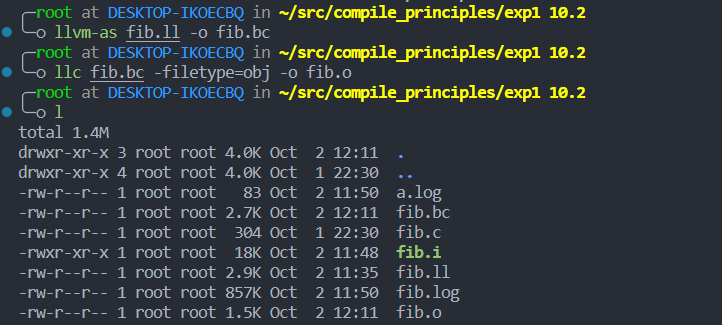
\includegraphics[width=\textwidth]{figure/output.png}
  \caption{汇编和链接 LLVM bitcode}
  \label{pic:6}
\end{figure}

对于生成的 fib.o 文件,使用如下命令对机器码进行反汇编得到 fib-anti-obj.S 文件,得到的反汇编结果如下:

\begin{minted}[linenos,frame=lines]{ASM}
fib.o:     file format elf64-x86-64

Disassembly of section .text:

0000000000000000 <main>:
0:  55                     push   %rbp
1:  48 89 e5               mov    %rsp,%rbp
4:  48 83 ec 20            sub    $0x20,%rsp
  8:  c7 45 e8 00 00 00 00   movl   $0x0,-0x18(%rbp)
f:  c7 45 f4 00 00 00 00   movl   $0x0,-0xc(%rbp)
  16:  c7 45 fc 01 00 00 00   movl   $0x1,-0x4(%rbp)
1d:  c7 45 f8 01 00 00 00   movl   $0x1,-0x8(%rbp)
  24:  48 bf 00 00 00 00 00   movabs $0x0,%rdi
2b:  00 00 00
2e:  48 8d 75 f0            lea    -0x10(%rbp),%rsi
32:  b0 00                  mov    $0x0,%al
  34:  e8 00 00 00 00         call   39 <main+0x39>
  39:  48 bf 00 00 00 00 00   movabs $0x0,%rdi
40:  00 00 00
43:  48 8d 75 f4            lea    -0xc(%rbp),%rsi
47:  b0 00                  mov    $0x0,%al
  49:  e8 00 00 00 00         call   4e <main+0x4e>
  4e:  48 bf 00 00 00 00 00   movabs $0x0,%rdi
55:  00 00 00
58:  48 8d 75 fc            lea    -0x4(%rbp),%rsi
5c:  b0 00                  mov    $0x0,%al
  5e:  e8 00 00 00 00         call   63 <main+0x63>
  63:  8b 45 f8               mov    -0x8(%rbp),%eax
  66:  3b 45 f0               cmp    -0x10(%rbp),%eax
  69:  7d 35                  jge    a0 <main+0xa0>
  6b:  8b 45 fc               mov    -0x4(%rbp),%eax
  6e:  89 45 ec               mov    %eax,-0x14(%rbp)
  71:  8b 45 f4               mov    -0xc(%rbp),%eax
  74:  03 45 fc               add    -0x4(%rbp),%eax
  77:  89 45 fc               mov    %eax,-0x4(%rbp)
  7a:  48 bf 00 00 00 00 00   movabs $0x0,%rdi
81:  00 00 00
84:  48 8d 75 fc            lea    -0x4(%rbp),%rsi
88:  b0 00                  mov    $0x0,%al
  8a:  e8 00 00 00 00         call   8f <main+0x8f>
  8f:  8b 45 ec               mov    -0x14(%rbp),%eax
  92:  89 45 f4               mov    %eax,-0xc(%rbp)
  95:  8b 45 f8               mov    -0x8(%rbp),%eax
  98:  83 c0 01               add    $0x1,%eax
9b:  89 45 f8               mov    %eax,-0x8(%rbp)
9e:  eb c3                  jmp    63 <main+0x63>
a0:  8b 45 e8               mov    -0x18(%rbp),%eax
a3:  48 83 c4 20            add    $0x20,%rsp
  a7:  5d                     pop    %rbp
  a8:  c3                     ret
  \end{minted}

对比原汇编代码 fib.S 文件可见,主体部分的代码完全一致,原文件中 label、无用的标记符号等被删去,得到了更为纯净的汇编代码。

\section{链接器做了什么}
由汇编程序生成的目标文件不能够直接执行。大型程序经常被分成多个部分进行编译,因此,可重定位的机器代码有必要和其他可重定位的目标文件以及库文件链接到一起,最终形成真正在机器上运行的代码。进而链接器对该机器代码进行执行生成可执行文件。
\verb|clang fib.o -o fib|

对可执行文件进行反汇编:\verb|objdump -d fib > fib-anti-exe.S|,得到的反汇编结果如下:

\begin{minted}[linenos,frame=lines]{ASM}

fib:     file format elf64-x86-64


Disassembly of section .init:

0000000000001000 <_init>:
1000:  48 83 ec 08            sub    $0x8,%rsp
  1004:  48 8b 05 c5 2f 00 00   mov    0x2fc5(%rip),%rax        # 3fd0 <__gmon_start__@Base>
  100b:  48 85 c0               test   %rax,%rax
  100e:  74 02                  je     1012 <_init+0x12>
  1010:  ff d0                  call   *%rax
  1012:  48 83 c4 08            add    $0x8,%rsp
1016:  c3                     ret

Disassembly of section .plt:

0000000000001020 <printf@plt-0x10>:
1020:  ff 35 ca 2f 00 00      push   0x2fca(%rip)        # 3ff0 <_GLOBAL_OFFSET_TABLE_+0x8>
1026:  ff 25 cc 2f 00 00      jmp    *0x2fcc(%rip)        # 3ff8 <_GLOBAL_OFFSET_TABLE_+0x10>
102c:  0f 1f 40 00            nopl   0x0(%rax)

0000000000001030 <printf@plt>:
1030:  ff 25 ca 2f 00 00      jmp    *0x2fca(%rip)        # 4000 <printf@GLIBC_2.2.5>
1036:  68 00 00 00 00         push   $0x0
  103b:  e9 e0 ff ff ff         jmp    1020 <_init+0x20>

  0000000000001040 <__isoc99_scanf@plt>:
  1040:  ff 25 c2 2f 00 00      jmp    *0x2fc2(%rip)        # 4008 <__isoc99_scanf@GLIBC_2.7>
  1046:  68 01 00 00 00         push   $0x1
104b:  e9 d0 ff ff ff         jmp    1020 <_init+0x20>

Disassembly of section .plt.got:

0000000000001050 <__cxa_finalize@plt>:
1050:  ff 25 8a 2f 00 00      jmp    *0x2f8a(%rip)        # 3fe0 <__cxa_finalize@GLIBC_2.2.5>
1056:  66 90                  xchg   %ax,%ax

Disassembly of section .text:

0000000000001060 <_start>:
1060:  31 ed                  xor    %ebp,%ebp
1062:  49 89 d1               mov    %rdx,%r9
1065:  5e                     pop    %rsi
1066:  48 89 e2               mov    %rsp,%rdx
1069:  48 83 e4 f0            and    $0xfffffffffffffff0,%rsp
  106d:  50                     push   %rax
  106e:  54                     push   %rsp
  106f:  45 31 c0               xor    %r8d,%r8d
  1072:  31 c9                  xor    %ecx,%ecx
  1074:  48 8d 3d d5 00 00 00   lea    0xd5(%rip),%rdi        # 1150 <main>
  107b:  ff 15 3f 2f 00 00      call   *0x2f3f(%rip)        # 3fc0 <__libc_start_main@GLIBC_2.34>
  1081:  f4                     hlt
  1082:  66 2e 0f 1f 84 00 00   cs nopw 0x0(%rax,%rax,1)
  1089:  00 00 00
  108c:  0f 1f 40 00            nopl   0x0(%rax)

  0000000000001090 <deregister_tm_clones>:
  1090:  48 8d 3d 89 2f 00 00   lea    0x2f89(%rip),%rdi        # 4020 <__TMC_END__>
  1097:  48 8d 05 82 2f 00 00   lea    0x2f82(%rip),%rax        # 4020 <__TMC_END__>
  109e:  48 39 f8               cmp    %rdi,%rax
  10a1:  74 15                  je     10b8 <deregister_tm_clones+0x28>
  10a3:  48 8b 05 1e 2f 00 00   mov    0x2f1e(%rip),%rax        # 3fc8 <_ITM_deregisterTMCloneTable@Base>
  10aa:  48 85 c0               test   %rax,%rax
  10ad:  74 09                  je     10b8 <deregister_tm_clones+0x28>
  10af:  ff e0                  jmp    *%rax
  10b1:  0f 1f 80 00 00 00 00   nopl   0x0(%rax)
  10b8:  c3                     ret
  10b9:  0f 1f 80 00 00 00 00   nopl   0x0(%rax)

  00000000000010c0 <register_tm_clones>:
  10c0:  48 8d 3d 59 2f 00 00   lea    0x2f59(%rip),%rdi        # 4020 <__TMC_END__>
  10c7:  48 8d 35 52 2f 00 00   lea    0x2f52(%rip),%rsi        # 4020 <__TMC_END__>
  10ce:  48 29 fe               sub    %rdi,%rsi
  10d1:  48 89 f0               mov    %rsi,%rax
  10d4:  48 c1 ee 3f            shr    $0x3f,%rsi
10d8:  48 c1 f8 03            sar    $0x3,%rax
  10dc:  48 01 c6               add    %rax,%rsi
  10df:  48 d1 fe               sar    %rsi
  10e2:  74 14                  je     10f8 <register_tm_clones+0x38>
  10e4:  48 8b 05 ed 2e 00 00   mov    0x2eed(%rip),%rax        # 3fd8 <_ITM_registerTMCloneTable@Base>
  10eb:  48 85 c0               test   %rax,%rax
  10ee:  74 08                  je     10f8 <register_tm_clones+0x38>
  10f0:  ff e0                  jmp    *%rax
  10f2:  66 0f 1f 44 00 00      nopw   0x0(%rax,%rax,1)
  10f8:  c3                     ret
  10f9:  0f 1f 80 00 00 00 00   nopl   0x0(%rax)

  0000000000001100 <__do_global_dtors_aux>:
  1100:  f3 0f 1e fa            endbr64
  1104:  80 3d 15 2f 00 00 00   cmpb   $0x0,0x2f15(%rip)        # 4020 <__TMC_END__>
110b:  75 2b                  jne    1138 <__do_global_dtors_aux+0x38>
110d:  55                     push   %rbp
110e:  48 83 3d ca 2e 00 00   cmpq   $0x0,0x2eca(%rip)        # 3fe0 <__cxa_finalize@GLIBC_2.2.5>
  1115:  00
  1116:  48 89 e5               mov    %rsp,%rbp
  1119:  74 0c                  je     1127 <__do_global_dtors_aux+0x27>
  111b:  48 8b 3d f6 2e 00 00   mov    0x2ef6(%rip),%rdi        # 4018 <__dso_handle>
  1122:  e8 29 ff ff ff         call   1050 <__cxa_finalize@plt>
  1127:  e8 64 ff ff ff         call   1090 <deregister_tm_clones>
  112c:  c6 05 ed 2e 00 00 01   movb   $0x1,0x2eed(%rip)        # 4020 <__TMC_END__>
1133:  5d                     pop    %rbp
1134:  c3                     ret
1135:  0f 1f 00               nopl   (%rax)
1138:  c3                     ret
1139:  0f 1f 80 00 00 00 00   nopl   0x0(%rax)

0000000000001140 <frame_dummy>:
1140:  f3 0f 1e fa            endbr64
1144:  e9 77 ff ff ff         jmp    10c0 <register_tm_clones>
1149:  0f 1f 80 00 00 00 00   nopl   0x0(%rax)

0000000000001150 <main>:
1150:  55                     push   %rbp
1151:  48 89 e5               mov    %rsp,%rbp
1154:  48 83 ec 20            sub    $0x20,%rsp
  1158:  c7 45 e8 00 00 00 00   movl   $0x0,-0x18(%rbp)
115f:  c7 45 f4 00 00 00 00   movl   $0x0,-0xc(%rbp)
  1166:  c7 45 fc 01 00 00 00   movl   $0x1,-0x4(%rbp)
116d:  c7 45 f8 01 00 00 00   movl   $0x1,-0x8(%rbp)
  1174:  48 bf 04 20 00 00 00   movabs $0x2004,%rdi
117b:  00 00 00
117e:  48 8d 75 f0            lea    -0x10(%rbp),%rsi
1182:  b0 00                  mov    $0x0,%al
  1184:  e8 b7 fe ff ff         call   1040 <__isoc99_scanf@plt>
  1189:  48 bf 04 20 00 00 00   movabs $0x2004,%rdi
1190:  00 00 00
1193:  48 8d 75 f4            lea    -0xc(%rbp),%rsi
1197:  b0 00                  mov    $0x0,%al
  1199:  e8 a2 fe ff ff         call   1040 <__isoc99_scanf@plt>
  119e:  48 bf 04 20 00 00 00   movabs $0x2004,%rdi
11a5:  00 00 00
11a8:  48 8d 75 fc            lea    -0x4(%rbp),%rsi
11ac:  b0 00                  mov    $0x0,%al
  11ae:  e8 8d fe ff ff         call   1040 <__isoc99_scanf@plt>
  11b3:  8b 45 f8               mov    -0x8(%rbp),%eax
  11b6:  3b 45 f0               cmp    -0x10(%rbp),%eax
  11b9:  7d 35                  jge    11f0 <main+0xa0>
  11bb:  8b 45 fc               mov    -0x4(%rbp),%eax
  11be:  89 45 ec               mov    %eax,-0x14(%rbp)
  11c1:  8b 45 f4               mov    -0xc(%rbp),%eax
  11c4:  03 45 fc               add    -0x4(%rbp),%eax
  11c7:  89 45 fc               mov    %eax,-0x4(%rbp)
  11ca:  48 bf 07 20 00 00 00   movabs $0x2007,%rdi
11d1:  00 00 00
11d4:  48 8d 75 fc            lea    -0x4(%rbp),%rsi
11d8:  b0 00                  mov    $0x0,%al
  11da:  e8 51 fe ff ff         call   1030 <printf@plt>
  11df:  8b 45 ec               mov    -0x14(%rbp),%eax
  11e2:  89 45 f4               mov    %eax,-0xc(%rbp)
  11e5:  8b 45 f8               mov    -0x8(%rbp),%eax
  11e8:  83 c0 01               add    $0x1,%eax
11eb:  89 45 f8               mov    %eax,-0x8(%rbp)
11ee:  eb c3                  jmp    11b3 <main+0x63>
11f0:  8b 45 e8               mov    -0x18(%rbp),%eax
11f3:  48 83 c4 20            add    $0x20,%rsp
  11f7:  5d                     pop    %rbp
  11f8:  c3                     ret

  Disassembly of section .fini:

  00000000000011fc <_fini>:
  11fc:  48 83 ec 08            sub    $0x8,%rsp
1200:  48 83 c4 08            add    $0x8,%rsp
1204:  c3                     ret
\end{minted}

可以发现所得结果长度大大增加,相较上一层新增了链接所得的内容。

\section{LLVM IR编程}
本次SysY语言特性研究,涵盖了函数,语句块,变量定义特性的程序例子编写和验证。

\subsection{变量定义}
此处定义了一个 int 类型变量、一个 int 类型指针、 一个 float 类型变量,并分别定义时赋值、赋值地址、定义后赋值。

\begin{minted}[linenos,frame=lines]{NASM}
@.str = private unnamed_addr constant [7 x i8] c"%d%p%f\00", align 1

define dso_local i32 @main() #0 {
  %1 = alloca i32, align 4
  %2 = alloca i32*, align 8
  %3 = alloca float, align 4
  store i32 1, i32* %1, align 4
  store i32* %1, i32** %2, align 8
  store float 2.500000e+00, float* %3, align 4
  %4 = load i32, i32* %1, align 4
  %5 = load i32*, i32** %2, align 8
  %6 = load float, float* %3, align 4
  %7 = fpext float %6 to double
  %8 = call i32 (i8*, ...) @printf(i8* noundef getelementptr inbounds ([7 x i8], [7 x i8]* @.str, i64 0, i64 0), i32 noundef %4, i32* noundef %5, double noundef %7)
  ret i32 0
}

declare i32 @printf(i8* noundef, ...) #1

\end{minted}

经过格式转换、汇编、链接,运行可执行程序可得正确输出结果如图\ref{pic:7}:
\begin{figure}[H]
  \centering
  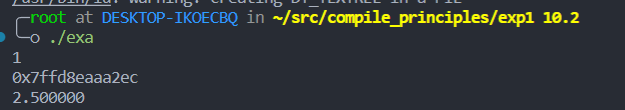
\includegraphics[width=\textwidth]{figure/exa.png}
  \caption{变量定义输出结果}
  \label{pic:7}
\end{figure}

\subsection{语句块}
此处我设计了一个普通语句块对变量进行修改和查看,并且设置了一个条件分支语句块和一个循环分支语句块。

\begin{minted}[linenos,frame=lines]{NASM}

@.str = private unnamed_addr constant [3 x i8] c"%d\00", align 1

define dso_local i32 @main() #0 {
  %1 = alloca i32, align 4
  %2 = alloca i32, align 4
  %3 = alloca i32, align 4
  %4 = alloca i32, align 4
  %5 = alloca i32, align 4
  %6 = alloca i32, align 4
  store i32 0, i32* %1, align 4
  store i32 1, i32* %3, align 4
  %7 = call i32 (i8*, ...) @__isoc99_scanf(i8* noundef getelementptr inbounds ([3 x i8], [3 x i8]* @.str, i64 0, i64 0), i32* noundef %2)
  store i32 0, i32* %5, align 4
  %8 = load i32, i32* %5, align 4
  %9 = call i32 (i8*, ...) @printf(i8* noundef getelementptr inbounds ([3 x i8], [3 x i8]* @.str, i64 0, i64 0), i32 noundef %8)
  %10 = load i32, i32* %3, align 4
  %11 = call i32 (i8*, ...) @printf(i8* noundef getelementptr inbounds ([3 x i8], [3 x i8]* @.str, i64 0, i64 0), i32 noundef %10)
  %12 = load i32, i32* %2, align 4
  %13 = icmp ne i32 %12, 0
  br i1 %13, label %14, label %27

  14:                                               ; preds = %0
  store i32 0, i32* %4, align 4
  store i32 1, i32* %6, align 4
  br label %15

  15:                                               ; preds = %23, %14
  %16 = load i32, i32* %6, align 4
  %17 = load i32, i32* %2, align 4
  %18 = icmp sle i32 %16, %17
  br i1 %18, label %19, label %26

  19:                                               ; preds = %15
  %20 = load i32, i32* %3, align 4
  %21 = load i32, i32* %4, align 4
  %22 = add nsw i32 %20, %21
  store i32 %22, i32* %4, align 4
  br label %23

  23:                                               ; preds = %19
  %24 = load i32, i32* %6, align 4
  %25 = add nsw i32 %24, 1
  store i32 %25, i32* %6, align 4
  br label %15, !llvm.loop !6

  26:                                               ; preds = %15
  br label %27

  27:                                               ; preds = %26, %0
  %28 = load i32, i32* %1, align 4
  ret i32 %28
}

declare i32 @__isoc99_scanf(i8* noundef, ...) #1

declare i32 @printf(i8* noundef, ...) #1

\end{minted}

经过格式转换、汇编、链接,运行可执行程序可得正确输出结果如图\ref{pic:8}:
\begin{figure}[H]
  \centering
  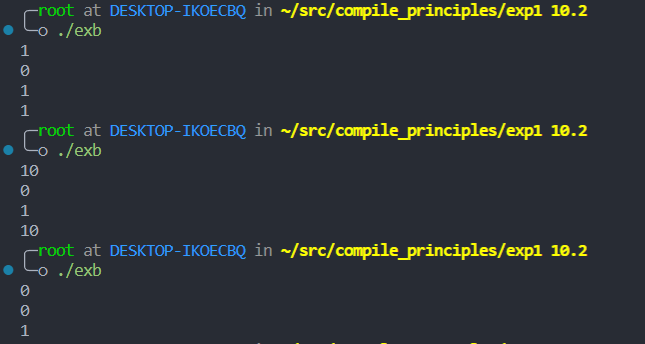
\includegraphics[width=\textwidth]{figure/exb.png}
  \caption{语句块输出结果}
  \label{pic:8}
\end{figure}

\subsection{函数}
这里设置了三个函数,一个返回 int 类型且不含参数,一个空类型且不含参数,一个返回 float 类型且含一个 int 类型参数。分别验证返回结果。
\begin{minted}[linenos,frame=lines]{NASM}

@b = dso_local global i32 0, align 4
@.str = private unnamed_addr constant [4 x i8] c"%d\0A\00", align 1
@.str.1 = private unnamed_addr constant [4 x i8] c"%f\0A\00", align 1

define dso_local i32 @f1() #0 {
  %1 = load i32, i32* @b, align 4
  ret i32 %1
}

define dso_local void @f2() #0 {
  store i32 1, i32* @b, align 4
  ret void
}

define dso_local float @f3(i32 noundef %0) #0 {
%2 = alloca i32, align 4
store i32 %0, i32* %2, align 4
%3 = load i32, i32* %2, align 4
%4 = sdiv i32 %3, 2
%5 = sitofp i32 %4 to float
ret float %5
}

define dso_local i32 @main() #0 {
  store i32 0, i32* @b, align 4
  %1 = call i32 @f1()
  %2 = call i32 (i8*, ...) @printf(i8* noundef getelementptr inbounds ([4 x i8], [4 x i8]* @.str, i64 0, i64 0), i32 noundef %1)
  call void @f2()
  %3 = load i32, i32* @b, align 4
  %4 = call i32 (i8*, ...) @printf(i8* noundef getelementptr inbounds ([4 x i8], [4 x i8]* @.str, i64 0, i64 0), i32 noundef %3)
  %5 = load i32, i32* @b, align 4
  %6 = call float @f3(i32 noundef %5)
  %7 = fpext float %6 to double
  %8 = call i32 (i8*, ...) @printf(i8* noundef getelementptr inbounds ([4 x i8], [4 x i8]* @.str.1, i64 0, i64 0), double noundef %7)
  ret i32 0
}

declare i32 @printf(i8* noundef, ...) #1

\end{minted}

经过格式转换、汇编、链接,运行可执行程序可得正确输出结果如图\ref{pic:9}:
\begin{figure}[H]
  \centering
  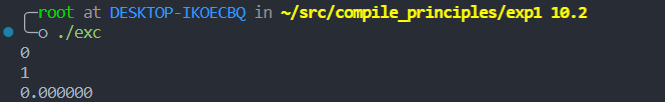
\includegraphics[width=\textwidth]{figure/exc.png}
  \caption{函数输出结果}
  \label{pic:9}
\end{figure}

\subsection{数组定义}

这里设计了不同维度,int和float类型的数组定义。

\begin{minted}[linenos,frame=lines]{NASM}
define dso_local i32 @main() #0 {
  %1 = alloca [2 x i32], align 4
  %2 = alloca [3 x [5 x i32]], align 16
  %3 = alloca [7 x [11 x [2 x i32]]], align 16
  %4 = alloca [13 x float], align 16
  %5 = alloca [2 x [4 x [6 x [10 x float]]]], align 16
  ret i32 0
}
\end{minted}

\subsection{隐式转换}

这里设计了int to float 和 float to int 两种隐式类型转换,等价SysY代码如下

\begin{minted}[linenos,frame=lines]{c}
int   i1 = 3.141592654;
int   i2 = 0.499999;
int   i3 = 0.500000;
int   i4 = 0.500001;
int   i5 = -0.499999;
int   i6 = -0.500000;
int   i7 = -0.500001;
float f1 = 3141592654;
float f2 = -314;
int   i8 = f1 / f2;
float f3 = i1 + i8;
\end{minted}

隐式转换中,字面常量会直接被编译器计算,float to int过程中会被截断小数部分,因此上述代码i2~i7均为0。int to float过程中按照IEEE 754规范转换,如果数字过大或过小会转换成inf。如果是没有在编译期确定的常量,会使用fptosi指令将浮点数转换成整数、sitofp指令将整数转换成浮点数。

\begin{minted}[linenos,frame=lines]{NASM}
define dso_local i32 @main() #0 {
  %1 = alloca i32, align 4
  %2 = alloca i32, align 4
  %3 = alloca i32, align 4
  %4 = alloca i32, align 4
  %5 = alloca i32, align 4
  %6 = alloca i32, align 4
  %7 = alloca i32, align 4
  %8 = alloca float, align 4
  %9 = alloca float, align 4
  %10 = alloca i32, align 4
  %11 = alloca float, align 4
  store i32 3, i32* %1, align 4
  store i32 0, i32* %2, align 4
  store i32 0, i32* %3, align 4
  store i32 0, i32* %4, align 4
  store i32 0, i32* %5, align 4
  store i32 0, i32* %6, align 4
  store i32 0, i32* %7, align 4
  store float 0x41E7681CC0000000, float* %8, align 4
  store float -3.140000e+02, float* %9, align 4
  %12 = load float, float* %8, align 4
  %13 = load float, float* %9, align 4
  %14 = fdiv float %12, %13
  %15 = fptosi float %14 to i32
  store i32 %15, i32* %10, align 4
  %16 = load i32, i32* %1, align 4
  %17 = load i32, i32* %10, align 4
  %18 = add nsw i32 %16, %17
  %19 = sitofp i32 %18 to float
  store float %19, float* %11, align 4
  ret i32 0
}
\end{minted}

\section{总结}
通过实战编写LLVM/IR程序,更深入地感受了语言处理系统各项完整的工作过程,熟悉了 LLVM IR 中间语言,并对其实现方式有了一定了解,为今后编写完整编译器打下良好基础。

\end{document}